\chapter{微积分: 导数}

\begin{figure}[ht]
  \centering
  \includegraphics[width=1\textwidth]{asset/茶桁的 AI 秘籍_Math_9.png}
\end{figure}

\newpage

我们终于结束了极限和连续的折磨, 开启了新的篇章. 

不过不要以为后面的就会很容易, 只是相对来说没有那么绕而已. 

那么, 我们今天开始学习「导数」. 

\section{导数}

在之前的导论, 也就是基础课里我们已经接触了导数. 在里面曾经提到, 「导数」和人工智能是最相关的一个概念. 我们再来回顾一下它的相关概念, 看看它的正式的定义是怎样的: 

\begin{align*}
  y' = \frac{dy}{dx} = f'(x) = \lim_{h \to 0} \frac{f(x+h) - f(x)}{(x+h) - x}
\end{align*}

来看这个定义, 一共三个等号. 其中$y'$、$\frac{dy}{dx}$、还有$f'(x)$, 都是导数的一种表示方式. 最后一个等号右边, 就是导数的正式定义, 当 h 趋近于 0 的时候, 在这个函数图像上分别取了两个点, 一个是$x$, 一个是$x+h$. 这两个点的距离不断缩小, 也就是当这个 h 不断趋近于 0 的时候, 函数图像上的这两点就几乎重合了. 

\begin{figure}[ht]
  \centering
  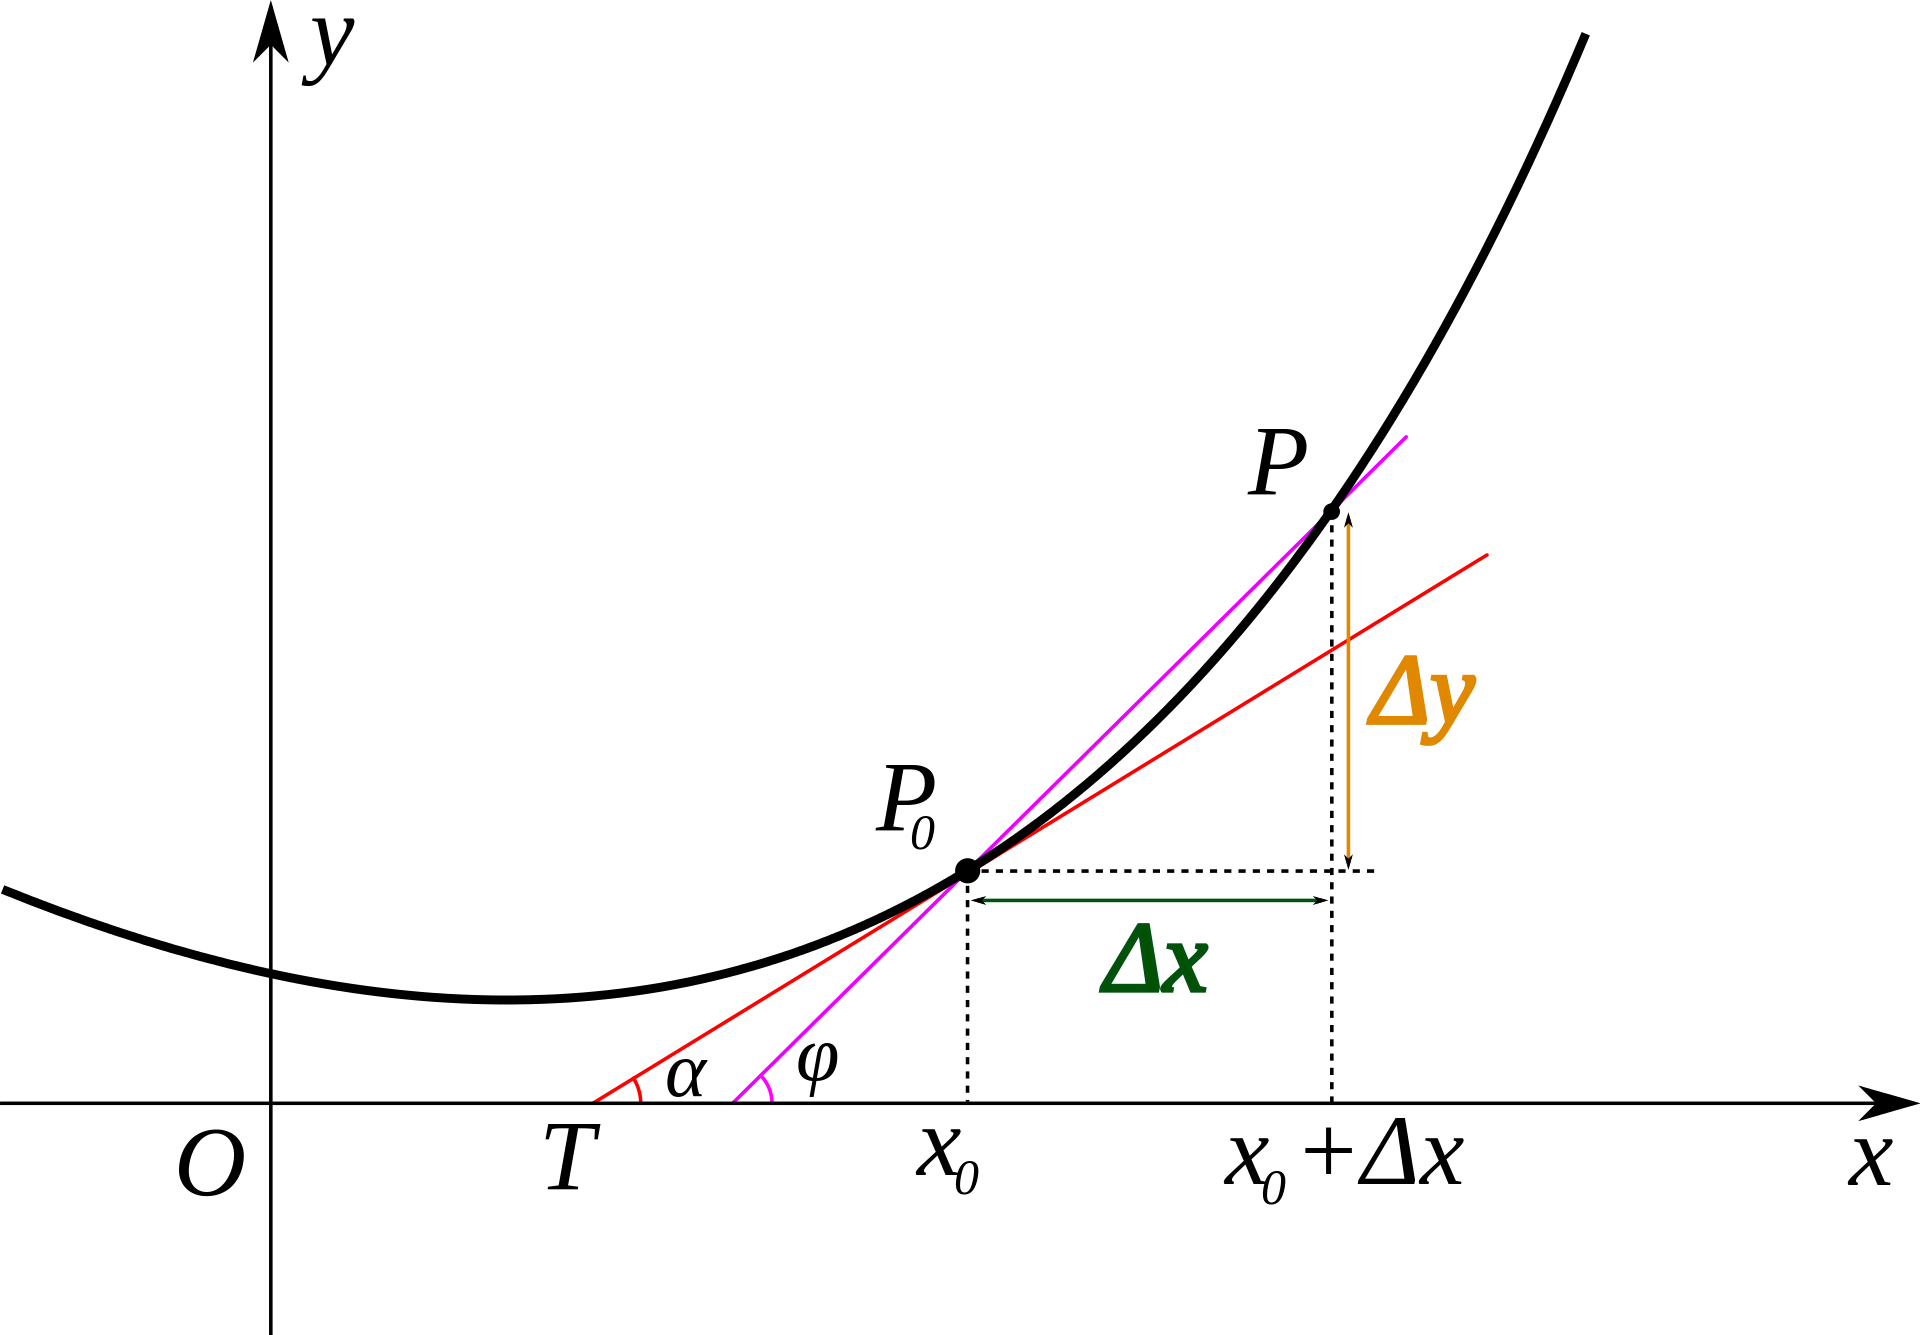
\includegraphics[width=0.5\textwidth]{asset/d46aa419-f50b-4bfd-83eb-d807f3c821a0.png}
  \caption{}
  \label{fig:img10_1}
\end{figure}

在之前的课程中我们也提到过. 这两点无限接近, 几乎重合的时候, 两点就归于一点了, 在上方图像中, 也就是$P_0$这一点. 这个点在函数图像上面就代表了一个切线, 也就是形成角$\alpha$的红色这条线. 所以, 导数的几何意义其实就是代表了这个函数图像上面一点的切线斜率, 并且代表了函数图像上这一点变化的快慢情况, 也就是这一点的变化率. 

任意函数的导数都可以通过这个定义式求解, 不过就是有的简单, 有的比较繁琐的而已. 前提是这个函数可导, 就是可求导. 它的这个导数可以按照我们定义的这个式子去做. 那问题来了, 有不可导的函数吗?

有, 而且还非常多. 说一个非常常见的,比如

\begin{align*}
  y=|x|, x \in R
\end{align*}

这个函数的函数图像如图:\ref{fig:img10_2}: 

\begin{figure}[ht]
  \centering
  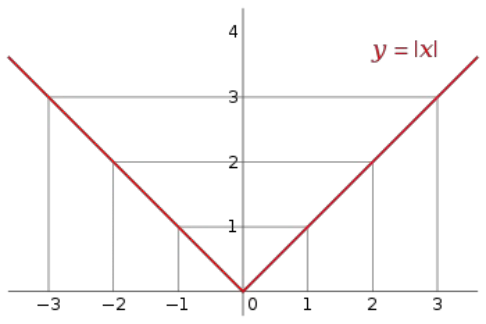
\includegraphics[width=0.5\textwidth]{asset/22572127-4cbd-4f9d-88bc-7ded3cd6940f.png}
  \caption{}
  \label{fig:img10_2}
\end{figure}

我们看这个函数, 首先, $x\in R$, R 代表的是实数集, $\in$表示的是属于, 也就是符号左边属于右边的集合, 它表示这种属于的关系. 

$y=|x|$可以写成分段函数的形式, 也就是下面这种形式: 

\begin{align*}
  y = f(x) =
  \begin{cases}
  -x, x<0 \\
  x, x \geq 0 \\
  \end{cases}
\end{align*}

当$x \geq 0$的时候,就是$x$本身, $x<0$的时候那就要添加一个负号, 负负得正. 

所以当我们单独的看这两个分段的时候, 我们会发现从 0 的左侧求导数的话, 结果是-1. 

因为我们说过导数的几何意义就是函数图像的切线斜率. 因为这条线就是一条直线, 那这上面的每一点的切线都和这条线本身重合. 所以这条线的斜率它就是-1. 

右边这一节的斜率就等于 1, 在这种情况下的话, 它的左导数等于-1, 他的右导数等于 1, 这两个不相等. 在同一个点 0 这里出现了矛盾. 左边说: 你得等于-1, 可是右边又说: 不行, 你得等于 1. 

所以在这种情况下它的导数本身在这点就产生了矛盾, 所以它的导数是不存在的, 我们把后面的推导补全, 就是: 

\begin{align*}
  & f'(x) = \begin{cases} -1, x<0 \\ 1, x \geq 0 \end{cases} \\
  & \mbox{从 0 的左侧求导数: } f'(0-) = -1, \\ 
  & \mbox{从 0 的有侧求导数: } f'(0+) = 1 \\ \\
  & f'(0-) \neq f'(0+)
\end{align*}

这个例子还是非常简单的, 大家应该都学过$y=|x|$的函数图像. 但就这么一个例子就能告诉我们导数不存在可以是长成什么样子的. 那从这个导数的例子里我们还可以得到一个什么结论?就是\textit{函数可导一定是连续的, 但是连续的不一定是可导的}. 

当然我们上一节导论课也已经说过很多关于导数的东西, 比如怎么样用定义去求一个东西的导数, 在导论课里面我们已经求了为什么正弦函数$sinx$导数是$cosx$, 大家如果忘记的话可以再回去看一下之前的课程\hyperlink{6.微积分-函数}{《6. 微积分 - 函数》}. 

\section{求导实例}

接下来, 我们看一下这个例子: 

\begin{figure}[ht]
  \centering
  \Large{例: 求函数 $y=x^x$ 的导数}
\end{figure}

现在我们要求导数, 怎么去求?在导论课里面我们上过哪些概念?我们当时有一个表列出了「常用函数的导数」对不对, 小伙伴们还记不记得?不记得也没关系, 我们这里再列一下.

\begin{table}
  \centering
  \begin{tabular}{ll}
    \midrule
      $C' = 0$ & $(x^n)' = nx^{n-1}$ \\
      $(sinx)' = cosx$ & $(cosx)' = -sinx$ \\
      $(a^x)' = a^x \ln a$ & $(e^x)' = e^x$ \\
      $(log_a{x})' = \frac{1}{x}log_a{e}$ &  $(\ln x)' = \frac{1}{x}$ \\
    \bottomrule
  \end{tabular}
  \caption{常用函数的导数}
  \label{fig:table10_1}
\end{table}

表\ref{fig:table10_1}中就是常用函数的导数, 似乎这里面没有我们可用的, 也就是通过常用函数的导数没法解. 

接下来, 我们再想想之前的课程还学过什么?之前还学过导数的一些运算法则, 来回忆一下: 

\paragraph{导数的运算法则}:

\begin{align*}
	\begin{split}
    & \mbox{设} u = u(x), v = v(x)\mbox{可导, 则: }\\ \\
    & (1) (u\pm v)' = u'\pm v' ; \\
    & (2) (cu)' = cu' (C\mbox{是常数}); \\
    & (3) (uv)' = u'v+uv'; \\
    & (4)(\frac{u}{v})' = \frac{u'v-uv'}{v^2}(v \ne 0)
	\end{split}
\end{align*}

可是在这种情况下似乎还是没有什么思路, 就是说$x^x$似乎并不是这四种组合里的其中一个, 所以这该怎么办?

这得费点脑子了, 让我们来一步一步看. 

首先, 两边同取对数. 对数运算大家应该都知道吧?比如说$3^2$, 这个结果等于多少?等于 9 对吧?

我们都知道$x^2$是一种乘方运算, 是针对指数的运算. 告诉你 3 的几次方, 都能算出来, 因为你知道 3 的平方等于两个 3 乘在一起, 3 的 3 次方等于 3 个 3 乘在一起. 

那我问你, 3 的 x 次方等于 9 你咋做?对数运算, 也就是刚才说的乘方运算反过来. 一个正一个反, 乘方运算是告诉你 3 的平方让你求结果. 对数运算就是 3 的多少次次方等于 9, 然后求它指数, 也就是它是几次方. 这就是对数的意思. 

如果小伙伴们还不太清楚, 可以自行 Google 一下. 这个太基础了, 就不多讲了. 我们接着来看当前这道题, 求$y=x^x$的导数. 

首先, 两边同取对数, 为什么两边同取一个对数?因为不管是什么样的运算, 只要等式两边是相等的, 不管做什么运算, 两边做同样的一个运算相等的结果仍然不会变.

\begin{align*}
  \ln y = x ln x
\end{align*}

$\ln y = x \cdot \ln x$, 其实是$\ln x^x$变化过来的. 对数运算有个特点, 就是 x 上面的指数部分可以拿在前面和它乘在一起. 所以这里是$x \cdot \ln x$.

接下来, 两边同时对 x 求导, 在这里关于导数的运算法则就可以用上了, 相当于是导数的嵌套.

因为 y 是关于 x 的函数, 所以两边先都关于 x 进行求导:

\begin{align*}
  \frac{d}{dx}(lny) = \frac{d}{dx}(xlnx) 
\end{align*}

左边咱们用链式法则来处理, 链式法则下节会讲, 这节课先知道这么用:

\begin{align*}
  \frac{d}{dx}(lny) = \frac{1}{y} \cdot \frac{dy}{dx} 
\end{align*}

这里的$\frac{dy}{dx}$就表示$y$对$x$的导数, 也就是$y'$, 所以就变成$\frac{1}{y} \cdot y'$, 也就是$\frac{y'}{y}$. 这是左边, 我们再来看右边. 

右边就是我们刚才那个导数运算法则里面的这个函数式$(uv)' = u'v+uv'$, 就是两个函数乘在一起求导, 分别等于其中一个求导再乘以另外一个, 之后将两者相加. 

我们来看, 先对 x 求导, x 求导就变成 1, $\ln x$不变拿过来, 就是$1 \cdot \ln x$, 然后再加上$\ln x$求导, 求导结果是$\frac{1}{x}$,  这次 x 不变拿过来. 我们就得到了这样一个式子: $1 \cdot \ln x + x \cdot \frac{1}{x}$. 再化简之后, 就得到了: $\ln x + 1$. 

最后我们就得到$\frac{y'}{y} = \ln x + 1$. 

继续, $y'$应该等于$y \cdot (\ln x + 1)$, 我们再把 y 用$x^x$代换一下, 最终我们得到$x^x(\ln x + 1)$. 

那我们最终是要求什么?是不是就是求$y'$, 那现在我们最终就得到了$y' = x^x(\ln x + 1)$为我们所求.

然后我要求大家去做的事就是大家可以自己去查一下对数、对数函数是怎么一回事, 以及它为什么有这样的性质: $ln x ^x$为什么就等于$x \ln x$. 也就是, 我们为什么可以将指数拿到前面去, 和对数函数相乘. 这部分应该是高中的内容. 

最后完整的推导过程就是: 

\begin{align*}
  & \frac{y'}{y} = 1 \cdot \ln x + x \cdot \frac{1}{x} \Rightarrow \frac{y'}{y} = \ln x + 1 \\ \\
  & \mbox{所以} y' = y(\ln x + 1) = x^x(\ln x + 1)
\end{align*}

接下来, 我们做一个比较有意思的事情, 我们做一个代码的演示. 上数学课这么久, 好久没接触代码了是不是?连我都有些小激动. 我们用代码来演示一下, 迭代法求解二次函数最小值, 来让我们开始: 

\section{代码演示: 迭代法求解二次函数最小值}

首先, 还是一样, 大家应该还记得如何导入需要的方法: 

\begin{python}
import numpy as np
import matplotlib.pyplot as plt
from IPython import display
\end{python}

在之前的 Python 课程中已经详细的讲解过 Python 的相关知识, 所以这里就不一一进行解释了. 

让我们先定义一个二次函数: 

\begin{python}
def f(x):
    y = x**2
    return y
\end{python}

紧接着, 我们还需要定义一个对应的导数: 

\begin{python}
# 定义对应的导数
def d(x):
    dy = 2*x
    return dy
\end{python}

这一步应该都看得懂吧?$y=x^2$对应的导数$y'$就应该等于$2x$. 

现在我们定义了两个自定义函数, 接下来希望将程序做成一个交互性的, 所以我们需要一个操作者输入指定的 x 初始值的操作: 

\begin{python}
# 操作者输入指定的 x 初始值
x = float(input('请输入 x 的初始值: '))
\end{python}

之后, 这段代码会给出一个动画的演示过程出来, 大家可以看得比较清楚我们是怎样在人工智能里面通过这种不断的迭代去求解一些神经网络的一个最优化的解. 

这里我们举一个比较简单的例子: 二次函数的最小值的求解过程. 

下面我们需要定义一个学习率, 并且准备一段二次函数数据点: 

\begin{python}
# 定义学习率
lr = 0.9

# 准备一段二次函数数据点
x_temp = np.linspace(-x, x, 1000)
y_temp = x_temp**2
\end{python}

\textbf{之后整个一段`while`循环, 都是为了输出图像的}, 之前我们学过`matplotlib`对吧, 这里就不详细的进行代码解释了, 大家下来可以执行研究一下代码, 我们主要是为了进行动画演示, 大家其实这里也不需要太了解, 不是主要目的: 

\begin{python}
while abs(x) > 0.01:
    # 用于清空之前的输出
    display.clear_output(wait = True) 
    # 清除之前的列表
    plt.clf()
    plt.plot(x_temp, y_temp)
    plt.scatter(x, f(x), s=30, c='red')
    plt.show()
    print('此时 x 的值为: ', x)
    plt.pause(0.7)
    \%matplotlib inline
    dy = d(x)
    x -= lr * dy
else:
    display.clear_output(wait=True)
    plt.clf()
    plt.plot(x_temp, y_temp)
    plt.scatter(x, f(x), s=30, c='red')
    plt.show()
    print('最终 x 的值为: ', x)
\end{python}


对于 y 等于 x 平方的二次函数. 我们要看它什么?先给它设一个起点, 比如说点 5 吧, 然后看它怎么样一步一步的逼近最小值点. 现在我们来看一下图\ref{fig:img10_3}: 

\begin{figure}[ht]
  \centering
  \includegraphics[width=0.5\textwidth]{asset/截屏 2023-12-31 12.45.38.png}
  \caption{动图无法正常显示, 点击\href{https://raw.githubusercontent.com/hivandu/notes/main/img/20230830160512.gif}{查看原图}}
  \label{fig:img10_3}
\end{figure}

从一开始的点, 一点一点迭代, 是不是越来越靠近最小支点了?就是这样一步一步的迭代, 直到达到我们要求的误差范围之内. 就是说我们给定了一个最小误差在多少以内, 当到达之后, 它就停止了. 我们设定的值是$0.01$, 所以它最终$x$的取值是 $0.009671406556917058$. 

这个就是整个过程, 大家不要看着似乎很简单, 其实人工智能, 或者严格意义上来说是神经网络怎么优化?就是这么优化. 随机初始化一些参数, 然后这些参数就从刚才我们类似于$x=5$的点一步一步通过迭代不断的逼近最优解. 不断的逼近直到达到一个范围之内, 而且在这里我们是可以定义学习率的. 大家应该看到我代码里设置了一个学习率`lr = 0.9`. 学习率就是我每一步走多远, 你比如说在这里是 0.9, 如果我们弄成 0.2 的话大家看一下会发生什么, \ref{fig:img10_4}: 

\begin{figure}[ht]
  \centering
  \includegraphics[width=0.4\textwidth]{asset/截屏 2023-12-31 12.50.40.png}
  \caption{动图无法正常显示, 点击\href{https://raw.githubusercontent.com/hivandu/notes/main/img/20230830160512.gif}{查看原图}}
  \label{fig:img10_4}
\end{figure}

整个过程中, 每一步走的比较慢. 所以他就不会像刚才一样每一步跨的比较大, 两边对称轴一直在反复晃, 现在的消息就是单侧逼近了. 所以, 其实不管你再怎么复杂的神经网络, 都是用求导反向传播, 然后通过乘上优化算法、设置学习率去做的. 不管多么复杂的原理其实都是这么简单. 

大家肯定会觉得很神奇, 有没有人会认为我在蒙你们?神经网络那么复杂的东西, 那么复杂的任务都可以胜任, 原理居然这么简单. 对, 就是这么简单, 只不过它复杂在哪?它的网络结构可以很多样化, 第二个是它的优化方法可以很复杂, 以及他是不是添加到一些其他的量. 这些都是需要我们去考虑去设计的, 但是最根本的核心就是上图演示的这么一个过程. 

所以大家不要觉得 AI 和我们离得非常远, 就是显得好像我们和 AI 触手不可及一样, 原理其实都很简单. 

就比如二八定律是一个非常朴实的一个定律, 不管是在经济学领域还是在其他领域, 我个人觉得都是很适用的. 就像神经网络, 如果你说原理的话, 我们花 20\%的时间可能就可以学到他 80\%的东西了, 但是如果我们要学比较深入的一些内容, 往深度去学的话, 为了剩下那么 20\%的内容可能我们得填上 80\%的时间. 

展示就先到这一步, 在神经网络里面去优化整个网络的这么一个过程. 

\section{阶}

这里再提一个概念, 就是大家可能会看到经常有个术语叫什么几阶导数, 其实阶是什么意思呢?几阶就是对函数求几次导. 比如我们看下面这个函数, 就是二阶导数: 

\begin{align*}
  f''(x) = (f'(x))'
\end{align*}

这里我们对其求了两次导, 所以「阶」的含义就是: 几阶就对函数求几次导. 

再比如我们看下面例子: 

\begin{align*}
  \mbox{例子: 已知函数} \quad f(x) = 3x^4 + 5x^3 + 6x + sinx, \mbox{求其一阶及二阶导数}
\end{align*}

一阶导数, 就直接对先求一次导, 按照我们的求导法则, 这里就不赘述了, 大家可以自己尝试下自己查表去算. 结果我放在下面: 

\begin{align*}
  \mbox{一阶导数: }f'(x) = 12x^3 + 15x^2 + 6 + cosx
\end{align*}

二阶导数什么意思呢?就又对一阶导数再求一次导, 把一阶导数看作是一个原函数, 然后再对他去进行一个求导. 

比如说$12x^3$, 3 拿下来和 12 乘在一起, 计算结果就是$36x^2$, 那之后的每一步也就非常清晰该怎么做了对吧?那结果就是: 

\begin{align*}
  \mbox{二阶导数: } f''(x) = 36x^2 + 30x - sinx
\end{align*}

理解原理之后, 拿常用函数的导数和求导公式过来套就可以了. 大家以后要多做练习. 
